\chapter{Ising model and complexity theory}

\section{Ising model}
Consider a simple, undirected graph $G = (V, E)$ with $N$ nodes labelled by consecutive natural numbers. With each node $i \in V$, we associate a dichotomous spin variable $s_i \in \{-1, 1\}$. To each edge $\{i, j\} \in E$, we assign an interaction strength $J_{ij}$ and to each node $i \in V$ we assign local magnetic field $h_i$. Here, all $J_{ij}$ and $h_i$ are real numbers. For such system, one can define the following energy function (Hamiltonian)
\begin{equation}
\label{eq:ising-hamiltonian}
H(\mathbf{s}) = \sum_{\langle i, j \rangle} J_{ij} s_i s_j +  \sum_{i=1}^N h_i s_i,
\end{equation}
where $\mathbf{s} = (s_i, \ldots, s_N)$ and the first sum runs over all edges in $E$\footnote{In the literature, the Ising Hamiltonian \eqref{eq:ising-hamiltonian} is often negated. However, definition provided here is consistent with the one used by D-Wave, and thus more suitable for use in this thesis}.
\begin{figure}
    \centering
    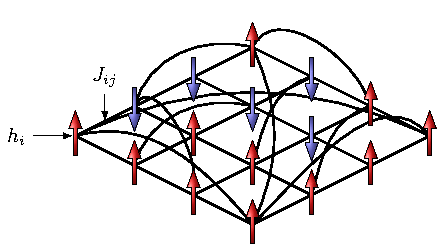
\includegraphics{figures/spins.pdf}
    \caption{An example of Ising  spin--glass defined on graph with $N=16$ nodes. Here, $h_i$ is a real number associated with $i$-th node, and $J_{ij}$ denotes coupling strength associated with edge between $i$-th and $j$-th node. Configuration of each spin is marked by a red arrow pointing upwards (+1) or a blue arrow pointing downwards (-1).}
    \label{fig:my_label}
\end{figure}
For fixed model coefficients, one is typically interested in finding its \emph{ground state}, a configuration $\mathbf{s}$ that minimizes $H$. More generally, it might be desirable to search for $k << 2^N$ configurations with lowest energy, the so called \emph{low--energy spectrum}.

The model was introduced in 1920 by Wilhelm Lenz \cite{lenz} as a description of ferromagnetism in solids, but is named after his student Ernst Ising, who studied and solved it in one-dimensional case \cite{ising}.  Despite the simple formulation, the problem of finding a ground state of Ising spin--glass is computationally hard \cite{barahoma}. Before expanding on this idea, let us first introduce hierarchy of complexity classes.

\section{Algorithms and complexity}
Solving computational problem requires suitable \emph{algorithm}, a description of steps to be performed by a computer in order to obtain a solution. It is hardly surprising that some problems might be solved in more than one way, i.e. there might exist different algorithms performing essentially the same task. Different algorithms solving the same problems might vastly differ in their demand on various resources, like memory or time needed to execute them. In practice, execution time (and usage of other resources) of given algorithm might also vary between its implementations, depending on factors like programming language or libraries used and the hardware it is executed on. Therefore, measuring execution time is not that useful in characterizing algorithm's performance.  Instead, it is more useful to characterize algorithms based on how their execution time scales (asymptotically) with increasing problem size. For instance, given an algorithm with execution time roughly proportional to the input size $N$, one might suspect that for problem instances large enough, it will perform better than the one with execution time proportional to $N^{2}$. This characteristics, known as computational complexity\footnote{Note that here we focus only on \emph{time complexity}, but other notions like memory complexity can be defined in similar fashion}, is formalized by a big-$O$ notation (see appendix for more detailed description). Using this notation, the algorithms from the above example would be classified as $O(N)$ and $O(N^{2})$ respectively. One might observe that the process of exhaustively searching through the whole state space of given Ising model requires at least $O(2^{N})$ time, since there are $2^{N}$ possible configurations to be examined. This observation already hints that the problem of finding the ground state is nontrivial.

\section{Complexity classes}
Althought there might exist multiple algorithms for solving given computational problem, one might consider the minimal time complexity required to do so. More generally, one might group computational problems based on their demand on resources (in some fixed model of computations). In this view, sets of similar problems are called \emph{complexity classes}. Definition of some complexity classes might also be restricted to specific types of problems. For instance, one might consider only decision problems, i.e. problems to which the answer is yes or no.

One of the fundamental complexity classes is \textbf{P}, a class of decision problems solvable in polynomial time on a deterministic Turing Machine. Another class, \textbf{NP}, comprises all decision problems solvable in polynomial time using a nondeterministic Turing Machine. It is interesting to note, that alternative characterization of \textbf{NP} class is as the one comprising all decision problems whose solution can be verified in polynomial time using deterministic Turing Machine. This is interesting not only from the theoretical standpoint, but also from the practical one. Namely, the second definition implies that to prove given problem is in \textbf{NP} it is enough to prove that the solution can be verified in polynomnial time on a deterministic Turing Machine.

One can immediately see that \textbf{P} $\subset$ \textbf{NP}. Indeed, if a problem is solvable in polynomial time, then it is also trivially verifiable in polynomial time. However, it is not immediately obvious if the inclusion is strict, and the question whether \textbf{P} $\ne$ \textbf{NP} is one of most imporant, yet unsolved problems in theoretical computer science.

The class of \textbf{NP--hard} problems comprises all the problems that are at least as hard as every problem in \textbf{NP}. More formally, given problem P is \textbf{NP--hard} if and only if solving every problem in \textbf{NP} can be reduced to solving P and then transforming the solution via some polynomial algorithm. Note that \textbf{NP--hard} class, contrary to \textbf{P} and \textbf{NP},  is not restricted to decision problems. In fact, it contains many optimization problems.

Problems in complexity class \textbf{P} are often considered tractable, or efficiently solvable, whereas problems not in \textbf{P} are perceived as hard and computationally demanding. However, this statement, known as Cobham's thesis, is imprecise, as it does not take into account multiple factors, including constant terms in big-O notation, or degrees of the involved polynomials. One can easily see that problem requiring $n^{10^6}$ time belongs to \textbf{P}, yet might be unsolvable even for very modest input of size $n=2$. This simple example demonstrates, that complexity classes can serve only as a rule of thumb when judging whether the problem at hand is tractable or not.

\begin{figure}
    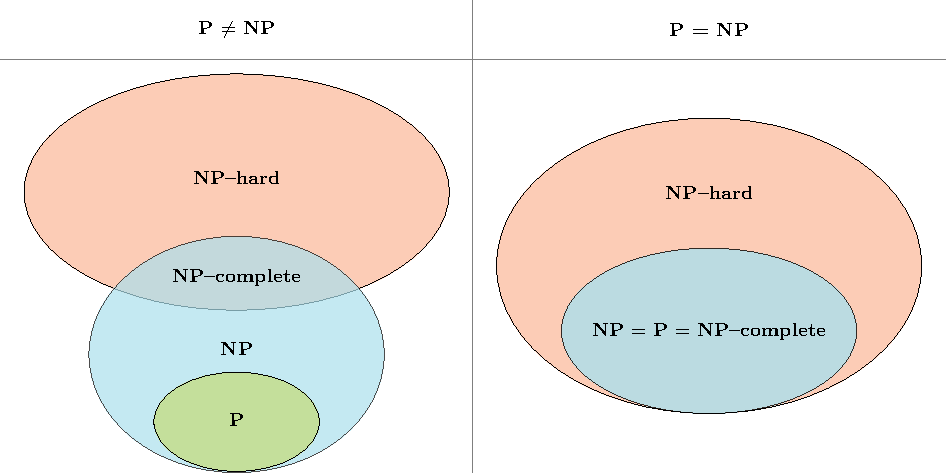
\includegraphics[width=\textwidth]{figures/complexity_new.pdf}
    \caption{Hierarchy of basic complexity classes under assumption of \textbf{P} $\ne$ \textbf{NP} (left) and \textbf{P} = \textbf{NP} (right). Notice that in both cases there exist \textbf{NP--hard} problems outside of \textbf{NP}.}
    \label{fig:complexity}
\end{figure}



\section{Overview of heuristic algorithms for solving Ising model}

As is the case with many NP--hard problems, there are many heuristic approaches for solving Ising model. One family of such algorithms relies on Metropolis-Hastings move for sampling from underlying Boltzmann distribution. In simulated annealing, one lowers temperature over time. Thus, the chance of accepting locally worse solution is greater at the start of the algorithm and decreases with each iteration, which helps avoiding getting stuck in local minimum. In another algorithm from the same family, \emph{parallel tempering}, one simulates several copies of the system, called replicas, in different temperatures. Neighbouring replicas are allowed to exchange states, with exchange probability depending on their energy and temperature difference. Replicas with the higher temperatures explore state space rapidly (thus reseeding the algorithm)., while ones with lower temperatures refine the best solutions found so far.

Most heuristic algorithms cannot certify the solution. \todo{Add info about cordial extensions}

%%% Local Variables:
%%% mode: latex
%%% TeX-master: "../main"
%%% End:
